\documentclass[12pt]{article}
\usepackage{graphicx}
\usepackage[none]{hyphenat}
\usepackage{graphicx}
\usepackage{listings}
\usepackage[english]{babel}
\usepackage{graphicx}
\usepackage{caption} 
\usepackage{booktabs}
\usepackage{array}
\usepackage{amssymb} % for \because
\usepackage{amsmath}   % for having text in math mode
\usepackage{extarrows} % for Row operations arrows
\usepackage{listings}
\lstset{
  frame=single,
  breaklines=true
}
\usepackage{hyperref}
  
%Following 2 lines were added to remove the blank page at the beginning
\usepackage{atbegshi}% http://ctan.org/pkg/atbegshi
\AtBeginDocument{\AtBeginShipoutNext{\AtBeginShipoutDiscard}}
\usepackage{gensymb}


%New macro definitions
\newcommand{\mydet}[1]{\ensuremath{\begin{vmatrix}#1\end{vmatrix}}}
\providecommand{\brak}[1]{\ensuremath{\left(#1\right)}}
\providecommand{\sbrak}[1]{\ensuremath{{}\left[#1\right]}}
\providecommand{\norm}[1]{\left\lVert#1\right\rVert}
\providecommand{\abs}[1]{\left\vert#1\right\vert}
\newcommand{\solution}{\noindent \textbf{Solution: }}
\newcommand{\myvec}[1]{\ensuremath{\begin{pmatrix}#1\end{pmatrix}}}
\let\vec\mathbf


\begin{document}

\begin{center}
	\title{\textbf{Gradient Descent}}
\date{\vspace{-5ex}} %Not to print date automatically
\maketitle
\end{center}
\setcounter{page}{1}

\section{12$^{th}$ Maths - Chapter 6}
This is Problem-23 from Exercise 6.6 
\begin{enumerate}
	\item Find the equation of the normal to the curve $x^2=4y$ and passing through the point $(1,2)$.

\solution 
The given equation of the curve can be written as  
\begin{align}
	\label{eq:parabolaEq2}
	g\brak{\vec{x}} = \vec{x}^T\vec{V}\vec{x} + 2\vec{u}^T\vec{x} + f = 0 
\end{align}
where
\begin{align}
	\label{eq:eqV}
	\vec{V} &= \myvec{ 1 & 0 \\ 0 & 0} \\
	\label{eq:eqU}
	\vec{u} &= \myvec{0 \\ -2} \\
	\label{eq:eqF}
	f &= 0 
\end{align}
We are given that 
\begin{align}
	\vec{h} &= \myvec{1 \\ 2}
\end{align}
This can be formulated as optimization problem as below:
\begin{align}
	\label{eq:Eq3}
	&  \min_{\vec{x}} \quad \text{f}\brak{\vec{x}} = \norm{\vec{x}-\vec{h}}^2\\
	\label{eq:Eq4}
	& \text{s.t.}\quad g\brak{\vec{x}} = \vec{x}^T\vec{V}\vec{x} + 2\vec{u}^T\vec{x} + f = 0  
\end{align}
It is already proved that the optimization problem is nonconvex. The constraints throw an error when \textit{cvxpy} is used. 

We will use Gradient Descent method to find the optimum value. Define
\begin{align}
	\label{eq:grad_des}
	x_{n+1} = x_n - \alpha \nabla g\brak{x_n} \\
	\text{ with loop condition as } \brak{\vec{x}-\vec{h}}^\top\nabla g\brak{x_n} \quad != 0 
\end{align}
Choosing
\begin{enumerate}
\item $\alpha$ = 0.001
\item precision = 0.001
\item n = 10000
\item $x_0$ = 4 
\end{enumerate}
\begin{align}
	\vec{x}_{min} &= \vec{q} = \myvec{ 2 \\1} 
\end{align}
Given the point of contact $\vec{q}$, the equation to the normal is given by
\begin{align}
	&\brak{\vec{V}\vec{q}+\vec{u}}^\top\vec{R}\brak{\vec{x}-\vec{q}} = 0 \\
	&\implies \brak{\myvec{1&0\\0&0}\myvec{2\\1}+\myvec{0 \\ -2}}^\top \myvec{0&1 \\-1&0}\brak{\vec{x}-\myvec{2\\1}} =0\\
	&\implies \myvec{2&-2} \myvec{0&1 \\-1&0}\brak{\vec{x}-\myvec{2\\1}} = 0 \\
	&\implies \myvec{2&2}\brak{\vec{x}-\myvec{2\\1}} = 0 \\
	&\implies \myvec{1&1}\vec{x} = 3 
\end{align}
The relevant figure is shown in \ref{fig:Fig1}
\begin{figure}[!h]
	\begin{center}
		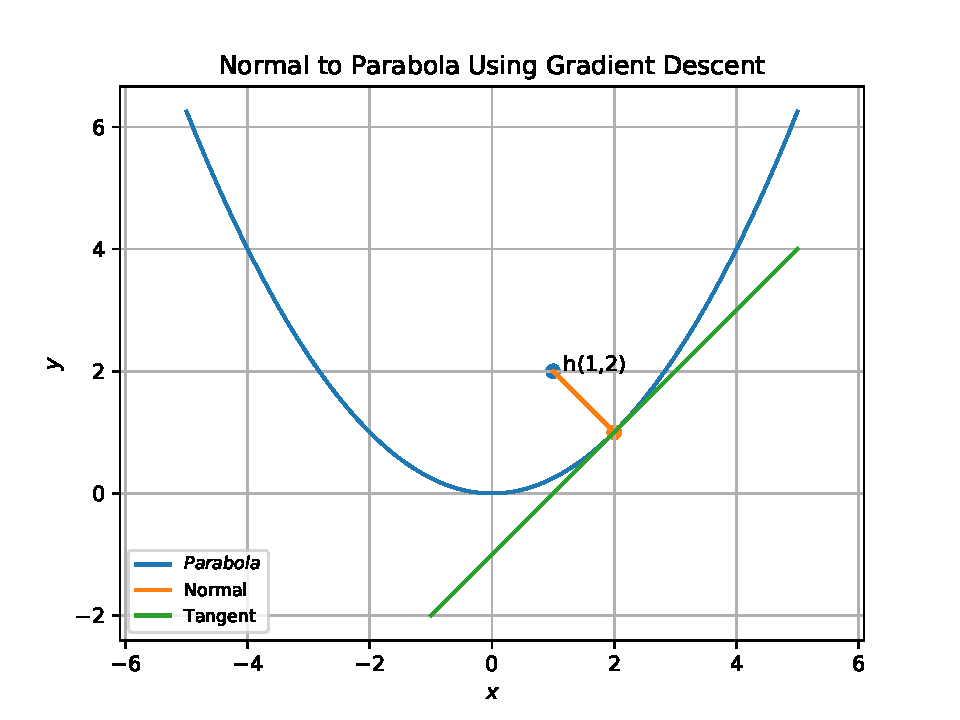
\includegraphics[width=\columnwidth]{figs/problem23.pdf}
	\end{center}
\caption{}
\label{fig:Fig1}
\end{figure}
\end{enumerate}
\end{document}
